\documentclass{beamer}
\beamertemplatenavigationsymbolsempty
\usepackage{amsmath, amssymb, hyperref, graphics, tikz}
%\usepackage{mathpazo, soul}



\newcommand{\C}{\mathbb{C}}
\newcommand{\Z}{\mathbb{Z}}
\newcommand{\R}{\mathbb{R}}
\newcommand{\N}{\mathbb{N}}
\DeclareMathOperator{\Real}{Re}
\DeclareMathOperator{\Imag}{Im}


\begin{document}

\begin{frame}{}
``From now on, we treat $f$ as the main function, and do not split into $\Real(f)$ and $\Imag(f)$.''

\includegraphics[width=\textwidth,height=0.8\textheight,keepaspectratio]{IsThisMeme.jpeg}
\end{frame}

\begin{frame}{Last time: Harmonic Functions}
The Laplacian operator, written $\nabla^2$ or $\Delta$, acts on functions $g:\R^2\to\R$ by
$$\nabla^2g=\nabla\cdot\nabla g=\frac{\partial^2 g}{\partial x^2}+\frac{\partial^2 g}{\partial y^2}$$
\begin{definition}
A function $u:\R^2\to\R$ is \emph{harmonic} if $\nabla^2f=0$.
\end{definition}

\begin{lemma}Let $f(z)=u(x,y)+iv(x,y)$ be analytic on a domain $D$.  Then $u$ and $v$ are harmonic on $D$.
\end{lemma}
\begin{block}{Can you go backwards?}
Yes, if $u$ defined on a \emph{simply-connected} region.  
\end{block}

\end{frame}

\begin{frame}{When is $u$ are the real part of analytic functions?}
\begin{block}{From the 2012-2013 exam}
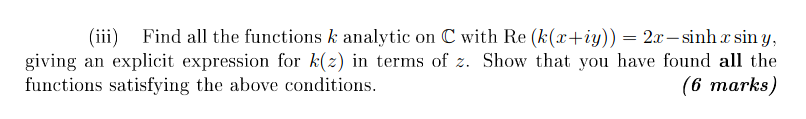
\includegraphics[width=\textwidth,height=0.8\textheight,keepaspectratio]{RealPart2012.png}
\end{block}

\begin{block}{The real part of an analytic function is harmonic}
First, check $\nabla^2u=0$.  If not, the answer is no.
\end{block}

\begin{block}{If it is, find $f^\prime$ using Cauchy-Riemann}
$$f^\prime=\frac{\partial}{\partial x} \Big(u(x,y)+iv(x,y)\Big)=u_x+iv_x=u_x-iu_y$$
\end{block}

This gives us $f^\prime$ in terms of $x$ and $y$.  We'd \emph{like} to write $f^\prime$ in terms of $z$, and integrate to find $f$. But how?

\begin{block}{Maybe we need a clever little trick....}
\end{block}

\end{frame}

\begin{frame}{Dr. Hart's "Clever little trick"}
\begin{block}{Given:}
We know $f^\prime$ in terms of $x$ and $y$, want it terms of $z$.
\end{block}

\begin{block}{Guess:}
Set $y=0$; to get $f^\prime(x)$ in terms of just $x$.  Integrate to get $f(x)$.  Guess that this is actually formula for $f(z)$
\end{block}

\begin{block}{Check:}
Show that $\Real(f)=u(x,y)$
\end{block}
\begin{block}{To find \emph{all} such $k$:}
\begin{lemma}Suppose that $f$ and $g$ are analytic on a region $D$ and that $\Real(f)=\Real(g)$ on $D$.  Then $f=g+ia$ for some $a\in\R.$
\end{lemma}
\end{block}

\end{frame}

\begin{frame}{A last application of Cauchy-Riemann}

\begin{itemize}
    \item Cauchy-Riemann relates between $\Real(f)$ and $\Imag(f)$
    \item If we have more relations, then $f$ is \emph{very} constrained
\end{itemize}

\begin{block}{Example from the notes:}
The function $f$ is analytic in $\C$ and its real and imaginary parts $u$ and $v$ satisfy 

$$ue^v=12$$ 
at all points in $\C$.  Prove that $f$ is constant.
\end{block}

\begin{block}{Next up -- Section 6: Power series}
\begin{itemize}
\item Not much different than real power series, so largely review
\item Spoiler: analytic functions have convergent power series 
\end{itemize}
\end{block}
\end{frame}




\end{document}
